\documentclass{article}
\usepackage[T1]{fontenc}
\usepackage{lmodern}
\usepackage{graphicx}
\usepackage{amsmath,amssymb}
\usepackage[a4paper,margin=2cm]{geometry}
\usepackage[absolute,overlay]{textpos}
\setlength{\TPHorizModule}{1mm}
\setlength{\TPVertModule}{1mm}
\usepackage[indonesian]{babel}
\usepackage{hyperref}
\setlength{\emergencystretch}{2em}
% unit: Halaman 19

\begin{document}

% === Halaman 19 (llm) ===

\vspace{209.98mm}

\section*{Run program}

% deskripsi: Screenshot terminal yang menunjukkan eksekusi program Python untuk enkripsi dan dekripsi Caesar Cipher, menampilkan input pesan 'Nomor telponku 08234654890', input kunci '189', hasil ciphertext yang terenkripsi, dan hasil plainteks setelah didekripsi kembali.
% bbox normalisasi: [0.0970, 0.1900, 0.7880, 0.8970]
\begin{textblock*}{145.11mm}(20.37mm,56.43mm)
\noindent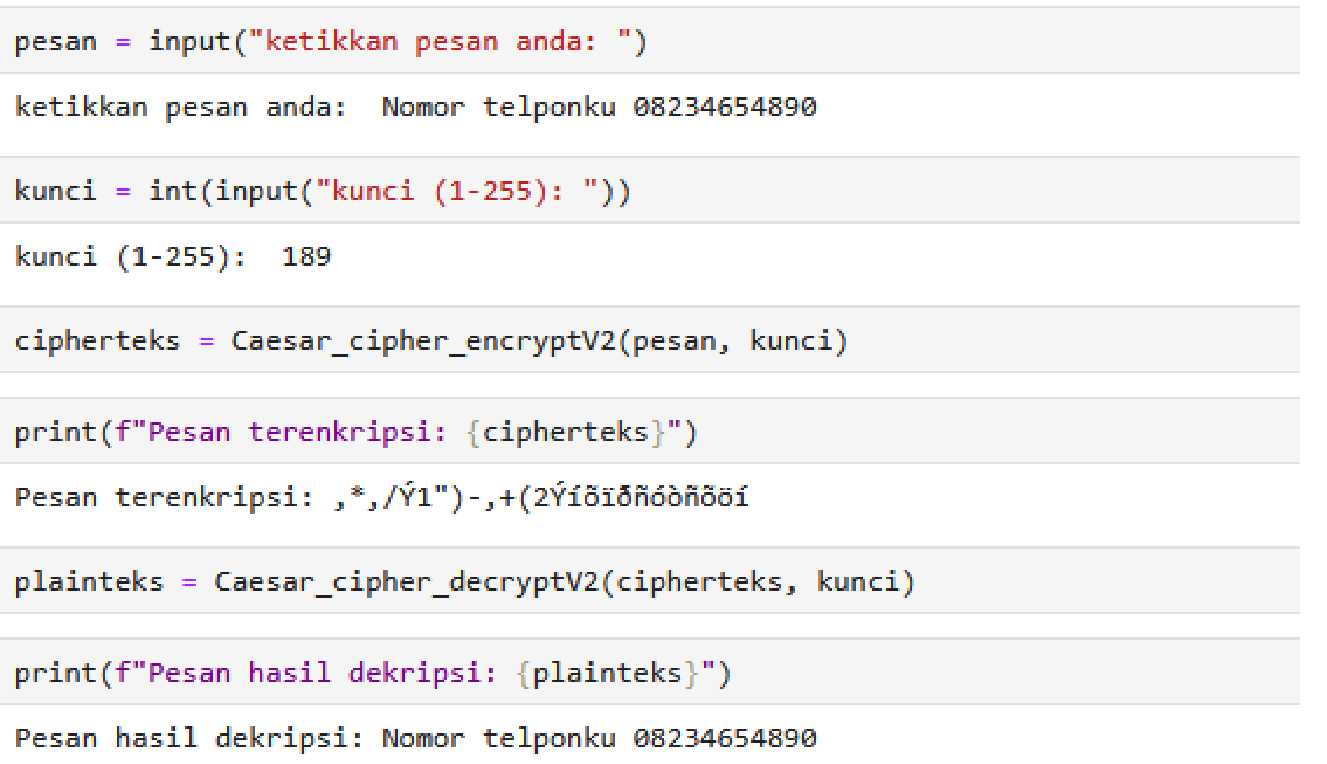
\includegraphics[width=145.11mm,height=209.98mm]{../../images/llm/page_019_img_01.png}%
\end{textblock*}

\end{document}
